\documentclass[]{report}
\usepackage{lmodern}
\usepackage{amssymb,amsmath}
\usepackage{ifxetex,ifluatex}
\usepackage{fixltx2e} % provides \textsubscript
\ifnum 0\ifxetex 1\fi\ifluatex 1\fi=0 % if pdftex
  \usepackage[T1]{fontenc}
  \usepackage[utf8]{inputenc}
\else % if luatex or xelatex
  \ifxetex
    \usepackage{mathspec}
  \else
    \usepackage{fontspec}
  \fi
  \defaultfontfeatures{Ligatures=TeX,Scale=MatchLowercase}
\fi
% use upquote if available, for straight quotes in verbatim environments
\IfFileExists{upquote.sty}{\usepackage{upquote}}{}
% use microtype if available
\IfFileExists{microtype.sty}{%
\usepackage{microtype}
\UseMicrotypeSet[protrusion]{basicmath} % disable protrusion for tt fonts
}{}
\usepackage[margin=1in]{geometry}
\usepackage{hyperref}
\hypersetup{unicode=true,
            pdfauthor={Samuel Lippl},
            pdfborder={0 0 0},
            breaklinks=true}
\urlstyle{same}  % don't use monospace font for urls
\usepackage{natbib}
\bibliographystyle{apalike}
\usepackage{color}
\usepackage{fancyvrb}
\newcommand{\VerbBar}{|}
\newcommand{\VERB}{\Verb[commandchars=\\\{\}]}
\DefineVerbatimEnvironment{Highlighting}{Verbatim}{commandchars=\\\{\}}
% Add ',fontsize=\small' for more characters per line
\usepackage{framed}
\definecolor{shadecolor}{RGB}{248,248,248}
\newenvironment{Shaded}{\begin{snugshade}}{\end{snugshade}}
\newcommand{\KeywordTok}[1]{\textcolor[rgb]{0.13,0.29,0.53}{\textbf{#1}}}
\newcommand{\DataTypeTok}[1]{\textcolor[rgb]{0.13,0.29,0.53}{#1}}
\newcommand{\DecValTok}[1]{\textcolor[rgb]{0.00,0.00,0.81}{#1}}
\newcommand{\BaseNTok}[1]{\textcolor[rgb]{0.00,0.00,0.81}{#1}}
\newcommand{\FloatTok}[1]{\textcolor[rgb]{0.00,0.00,0.81}{#1}}
\newcommand{\ConstantTok}[1]{\textcolor[rgb]{0.00,0.00,0.00}{#1}}
\newcommand{\CharTok}[1]{\textcolor[rgb]{0.31,0.60,0.02}{#1}}
\newcommand{\SpecialCharTok}[1]{\textcolor[rgb]{0.00,0.00,0.00}{#1}}
\newcommand{\StringTok}[1]{\textcolor[rgb]{0.31,0.60,0.02}{#1}}
\newcommand{\VerbatimStringTok}[1]{\textcolor[rgb]{0.31,0.60,0.02}{#1}}
\newcommand{\SpecialStringTok}[1]{\textcolor[rgb]{0.31,0.60,0.02}{#1}}
\newcommand{\ImportTok}[1]{#1}
\newcommand{\CommentTok}[1]{\textcolor[rgb]{0.56,0.35,0.01}{\textit{#1}}}
\newcommand{\DocumentationTok}[1]{\textcolor[rgb]{0.56,0.35,0.01}{\textbf{\textit{#1}}}}
\newcommand{\AnnotationTok}[1]{\textcolor[rgb]{0.56,0.35,0.01}{\textbf{\textit{#1}}}}
\newcommand{\CommentVarTok}[1]{\textcolor[rgb]{0.56,0.35,0.01}{\textbf{\textit{#1}}}}
\newcommand{\OtherTok}[1]{\textcolor[rgb]{0.56,0.35,0.01}{#1}}
\newcommand{\FunctionTok}[1]{\textcolor[rgb]{0.00,0.00,0.00}{#1}}
\newcommand{\VariableTok}[1]{\textcolor[rgb]{0.00,0.00,0.00}{#1}}
\newcommand{\ControlFlowTok}[1]{\textcolor[rgb]{0.13,0.29,0.53}{\textbf{#1}}}
\newcommand{\OperatorTok}[1]{\textcolor[rgb]{0.81,0.36,0.00}{\textbf{#1}}}
\newcommand{\BuiltInTok}[1]{#1}
\newcommand{\ExtensionTok}[1]{#1}
\newcommand{\PreprocessorTok}[1]{\textcolor[rgb]{0.56,0.35,0.01}{\textit{#1}}}
\newcommand{\AttributeTok}[1]{\textcolor[rgb]{0.77,0.63,0.00}{#1}}
\newcommand{\RegionMarkerTok}[1]{#1}
\newcommand{\InformationTok}[1]{\textcolor[rgb]{0.56,0.35,0.01}{\textbf{\textit{#1}}}}
\newcommand{\WarningTok}[1]{\textcolor[rgb]{0.56,0.35,0.01}{\textbf{\textit{#1}}}}
\newcommand{\AlertTok}[1]{\textcolor[rgb]{0.94,0.16,0.16}{#1}}
\newcommand{\ErrorTok}[1]{\textcolor[rgb]{0.64,0.00,0.00}{\textbf{#1}}}
\newcommand{\NormalTok}[1]{#1}
\usepackage{longtable,booktabs}
\usepackage{graphicx,grffile}
\makeatletter
\def\maxwidth{\ifdim\Gin@nat@width>\linewidth\linewidth\else\Gin@nat@width\fi}
\def\maxheight{\ifdim\Gin@nat@height>\textheight\textheight\else\Gin@nat@height\fi}
\makeatother
% Scale images if necessary, so that they will not overflow the page
% margins by default, and it is still possible to overwrite the defaults
% using explicit options in \includegraphics[width, height, ...]{}
\setkeys{Gin}{width=\maxwidth,height=\maxheight,keepaspectratio}
\IfFileExists{parskip.sty}{%
\usepackage{parskip}
}{% else
\setlength{\parindent}{0pt}
\setlength{\parskip}{6pt plus 2pt minus 1pt}
}
\setlength{\emergencystretch}{3em}  % prevent overfull lines
\providecommand{\tightlist}{%
  \setlength{\itemsep}{0pt}\setlength{\parskip}{0pt}}
\setcounter{secnumdepth}{5}

%%% Use protect on footnotes to avoid problems with footnotes in titles
\let\rmarkdownfootnote\footnote%
\def\footnote{\protect\rmarkdownfootnote}

%%% Change title format to be more compact
\usepackage{titling}

% Create subtitle command for use in maketitle
\newcommand{\subtitle}[1]{
  \posttitle{
    \begin{center}\large#1\end{center}
    }
}

\setlength{\droptitle}{-2em}

  \title{}
    \pretitle{\vspace{\droptitle}}
  \posttitle{}
    \author{Samuel Lippl}
    \preauthor{\centering\large\emph}
  \postauthor{\par}
      \predate{\centering\large\emph}
  \postdate{\par}
    \date{2018-09-13}

\usepackage{booktabs, titlesec, blindtext}
\usepackage[svgnames]{xcolor}
\hypersetup{
    bookmarksnumbered=true,
    bookmarksopen=false,
    bookmarksopenlevel=1,
    colorlinks=true,
    linkcolor=blue,
    urlcolor=DarkBlue,
    citecolor=DarkRed
}
\definecolor{chgray}{gray}{0.5}
\newcommand{\hsp}{\hspace{20pt}}
\titleformat{\chapter}[hang]{\Huge\bfseries}{\thechapter\hsp\textcolor{chgray}{|}\hsp}{0pt}{\Huge\bfseries}

\usepackage{amsthm}
\newtheorem{theorem}{Theorem}[chapter]
\newtheorem{lemma}{Lemma}[chapter]
\theoremstyle{definition}
\newtheorem{definition}{Definition}[chapter]
\newtheorem{corollary}{Corollary}[chapter]
\newtheorem{proposition}{Proposition}[chapter]
\theoremstyle{definition}
\newtheorem{example}{Example}[chapter]
\theoremstyle{definition}
\newtheorem{exercise}{Exercise}[chapter]
\theoremstyle{remark}
\newtheorem*{remark}{Remark}
\newtheorem*{solution}{Solution}
\begin{document}

\begin{titlepage}

% Titlepage inspired by: https://www.overleaf.com/15991102jmmvbxxtbhfk#/61015645/

\newcommand{\HRule}{\rule{\linewidth}{0.5mm}} % Defines a new command for the horizontal lines, change thickness here

\center % Center everything on the page

%----------------------------------------------------------------------------------------
%	TITLE SECTION
%----------------------------------------------------------------------------------------

\HRule \\[0.4cm]
{ \huge \bfseries Description, implementation and validation of a user interface for complex datasets in the social sciences}\\[0.4cm] % Title of your document
\HRule \\[1.5cm]

%----------------------------------------------------------------------------------------
%	HEADING SECTIONS
%----------------------------------------------------------------------------------------

\textsc{\LARGE Ludwig-Maximilians-Universität München}\\[0.5cm] % Name of your university/college
\textsc{\Large Fakultät für Mathematik, Informatik und Statistik}\\[1.5cm]


\textsc{\Large Bachelor of Statistics}\\[0.5cm] % Major heading such as course name
\textsc{\large Bachelor's Thesis}\\[0.5cm] % Minor heading such as course title

%----------------------------------------------------------------------------------------
%	LOGO SECTION
%----------------------------------------------------------------------------------------

\vfill


\includegraphics[height=0.2\textheight]{figs/sigill.png}\\[1cm] % Include a department/university logo - this will require the graphicx package



%----------------------------------------------------------------------------------------
%	DATE SECTION
%----------------------------------------------------------------------------------------

\vfill

%----------------------------------------------------------------------------------------
%	AUTHOR SECTION
%----------------------------------------------------------------------------------------

{\Large 30. Juni 2018}\\[1cm]
\begin{Large}
\textsc{Author}\\Samuel Lippl\\[1cm]
\textsc{Supervisor}\\
Dr. Fabian Scheipl
\end{Large}

\vfill

\end{titlepage}

\pagenumbering{roman}
\setcounter{page}{2}

\chapter*{Selbständigkeitserklärung}

Ich erkläre hiermit, dass ich die vorliegende Arbeit selbständig angefertigt, alle Zitate als solche kenntlich gemacht sowie alle benutzten Quellen und Hilfsmittel angegeben habe.\\

\begin{tabular}{c}
\\\\\\
\\\hline
Samuel Lippl, 15.09.2018
\end{tabular}

\chapter*{Abstract}\label{abstract}


This report will provide an overview over outlier detection in R. It
starts by discussing some general principles of outlier detection.
Linear methods and their nonlinear extensions are presented next. Along
the general methods, examples of application and an appropriate
methodology in R are introduced. The report will be concluded by a
discussion of method evaluation as well as a comparison of the different
introduced algorithms.

\tableofcontents

\chapter{Introduction}\label{intro}

\pagenumbering{arabic} \setcounter{page}{1}

One of the main advantages of the statistical programming language R
\citep{R} lies in its conciseness. With just one line of code, it is
possible to build a linear model, visualize a variable's distribution or
conduct complex modifications on several datasets. This is possible
because R is a domain-specific language and is therefore able to make
strong assumptions -- many people will need to build a linear model or
read in a csv file and it is therefore sensible to create custom
functions for these purpose.

An important property of this conciseness is that the code is still easy
to read. Two features that are especially important for this both rely
on the specific domain of statistical analysis for which R was created:

\begin{itemize}
\item
  \emph{Specialized functions:} \texttt{read.csv} essentially calls
  \texttt{read.table} with a few modified parameters. Nonetheless, it is
  immediately clear what this line of code is supposed to achieve.
\item
  \emph{Default values:} The user does not need to specify every single
  parameter of a function. For instance, it is helpful that
  \texttt{read.table} contains the parameter \texttt{na.strings} that
  allows the user to specify values that encode \texttt{NA}s. However,
  in most cases, \texttt{NA}s are encoded by the string \texttt{NA} or a
  missing value {[}\^{}1{]}. By setting default values, the user only
  needs to think about this parameter when the file structure is out of
  the ordinary.
\end{itemize}

{[}\^{}1:{]} The latter is only implemented in \texttt{read\_delim} from
the package \texttt{readr} but the advantage of default values remains
valid nevertheless.

These advantages are certainly not unique to R. They are designed to
minimize the expected time a user needs to spend with coding his
decisions while maintaining easy reproducibility of his work. On the
other hand, if there are more complicated tasks to undertake, a
consistent interface allows the user to do that, as well.

A good example for this concept, in my mind, is the package
\texttt{stringr} \citep{stringr}. Functions like \texttt{str\_trim}
(trim whitespace) or \texttt{str\_to\_title} (capitalize) make special
use cases easily accessible. On the other hand, \texttt{str\_replace}
allows more complicated operations with regular expressions using the
same consistent interface.

Things, however, start to fall apart when one attempts to modify default
values. This is possible by setting the global options in R; however,
relying on these makes reproducibility harder. On the other hand, one
could write new functions to solve this problem. This is, however, more
laborious than such an endeavour needs to be.

A good example of this are datasets with many variables as they occur in
the social sciences. As an example, I will consider the Varieties of
Democracy \href{V-DEM}{v-dem.net} dataset which produces indicators of
democracy \citep[\citet{Pemstein2018}]{vdem2018}. It contains many
variables on different aspects of democracy with values per country and
year. If one wishes to visualize the development of this variable over
time, a simple line plot often makes sense. Consider, for instance, the
variable which characterizes the freedom of religion on a scale between
0 and 4 for Germany:

\begin{Shaded}
\begin{Highlighting}[]
\NormalTok{df_vdem }\OperatorTok\StringTok{ }
\StringTok{  }\KeywordTok{filter}\NormalTok{(country_name }\OperatorTok{==}\StringTok{ "Germany"}\NormalTok{) }\OperatorTok\StringTok{ }
\StringTok{  }\KeywordTok{ggplot}\NormalTok{(}\KeywordTok{aes}\NormalTok{(year, v2clacfree_osp)) }\OperatorTok{+}\StringTok{ }
\StringTok{  }\KeywordTok{geom_line}\NormalTok{()}
\end{Highlighting}
\end{Shaded}

\begin{figure}
\centering
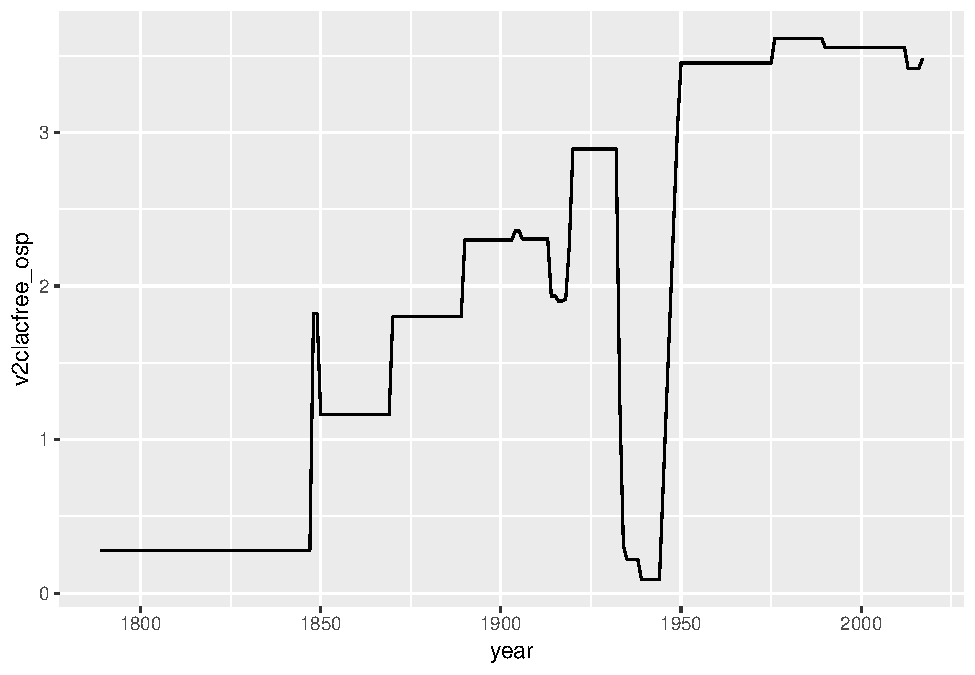
\includegraphics{bachelor-thesis_files/figure-latex/ex1-1.pdf}
\caption{\label{fig:ex1}Example: Freedom of religion in Germany over time}
\end{figure}

Although there are considerable changes within a single year, freedom of
religion is a continuous value and linear interpolation of this
development within a year makes sense.

Considering the variable \texttt{v2elvotbuy\_osp}, however, a line plot
makes less sense. This variable captures whether there was evidence of
vote buying during a national election and is therefore only present in
years where there has been a national election. A step plot seems more
sensible in this case as the represented value would always refer to the
last election.

\begin{Shaded}
\begin{Highlighting}[]
\NormalTok{df_vdem }\OperatorTok\StringTok{ }
\StringTok{  }\KeywordTok{filter}\NormalTok{(country_name }\OperatorTok{==}\StringTok{ "Germany"}\NormalTok{) }\OperatorTok\StringTok{ }
\StringTok{  }\KeywordTok{select}\NormalTok{(year, v2elvotbuy_osp) }\OperatorTok\StringTok{ }
\StringTok{  }\KeywordTok{na.omit}\NormalTok{() }\OperatorTok\StringTok{ }
\StringTok{  }\KeywordTok{ggplot}\NormalTok{(}\KeywordTok{aes}\NormalTok{(year, v2elvotbuy_osp)) }\OperatorTok{+}\StringTok{ }\KeywordTok{geom_step}\NormalTok{()}
\end{Highlighting}
\end{Shaded}

\begin{figure}
\centering
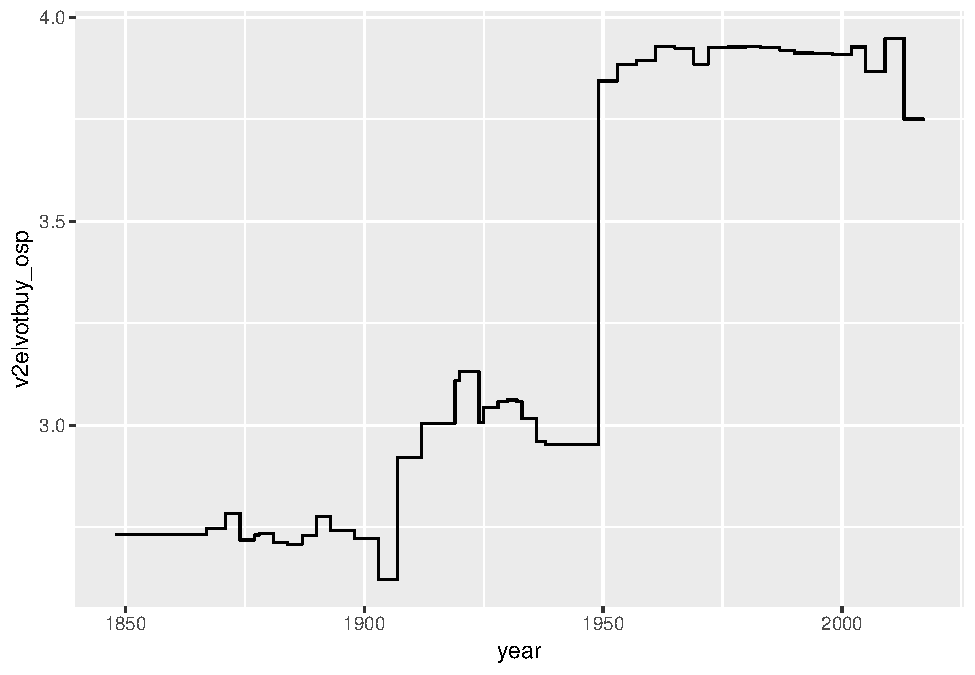
\includegraphics{bachelor-thesis_files/figure-latex/ex2-1.pdf}
\caption{\label{fig:ex2}Example: Election vote buying in Germany over time}
\end{figure}

Furthermore, the scale titles should be modified to show an
interpretable variable name, the scale should in many be standardized to
depict the entire range between 0 and 4.

In summary, there are many considerations one needs to implement in such
a visualization. Therefore, every time the statistician needs to
implement such a visualization, she needs to think about these questions
again, which is time expensive and makes interactive user interfaces
impossible. This problem is not limited to visualization; another
example would be descriptive tables of a linear model or a report
summarizing all covariates that have been used.

In summary, R provides amazing opportunities to to outsource everyday
thought processes in data analysis. However, adapting these mechanisms
for application-specific thought processes is expensive and difficult. A
broad framework for such an adaptation would enable researchers to think
about certain decisions (like the visualization of a specific variable)
once and then be done with it. Both the researcher himself and his
colleagues who might not need to think about this at all would benefit
from this.

In this Bachelor's Thesis, I describe such a framework, implement it as
the package \texttt{tectr} in R and apply it to the V-DEM dataset. The
\href{next\%20chapter}{\#methods} discusses some details regarding the
package construction and the dataset before we get a
\href{first\%20look}{\#example} in the third chapter. The
\href{fourth\%20chapter}{\#concept} will present the framework and the
implementation in a more specific way.
\href{Chapter\%20five}{\#application} presents the application of
\texttt{tectr} to the V-DEM dataset and the
\href{final\%20chapter}{\#summary} summarizes the thesis and discusses
the next steps regarding \texttt{tectr}.

\chapter{Methodology}\label{methods}

This chapter introduces the V-DEM dataset and discuss the methodological
background of \texttt{tectr}'s construction.

\section{V-DEM}\label{v-dem}

\subsection{Introduction to the
database}\label{introduction-to-the-database}

The Varieties of Democracy Institute is concerned with measuring
different aspects of democracy. It distinguishes between seven
high-level principles: electoral, liberal, participatory, deliberative,
egalitarian, majoritarian and consensual. These are measured by a
variable in the interval \([0,1]\) and consist of several mid- and
low-level indices. The low-level indices are coded with the help of
several country experts. These receive a questionnaire. Most questions
can be answered by an ordinal scale of five alternatives. Consider, as
an example, the variable ``Disclosure of campaign donations'':

\begin{quote}
\emph{Question}: Are there disclosure requirements for donations to
national election campaigns? 0: No. There are no disclosure
requirements. 1: Not really. There are some, possibly partial,
disclosure requirements in place but they are not observed or enforced
most of the time. 2: Ambiguous. There are disclosure requirements in
place, but it is unclear to what extent they are observed or enforced.
3: Mostly. The disclosure requirements may not be fully comprehensive
(some donations not covered), but most existing arrangements are
observed and enforced. 4: Yes. There are comprehensive requirements and
they are observed and enforced almost all the time.
\end{quote}

The answers are then analyzed for inter-coder reliability and a
standardized average of the responses together with a confidence
interval which contains 68 \% of the probability mass is created.
Lower-level indices are created from these answers which are summarized
in mid-level and then high-level indices. An overview over the structure
can be found in appendix D of the codebook \citep{vdem-codebook2018}.
The database contains data on 201 countries between 1789 and 2017.
\citep[\citet{Pemstein2018}]{vdem2018}

\subsection{\texorpdfstring{\texttt{vdem.tectr}}{vdem.tectr}}\label{vdem.tectr}

I have created the package \texttt{vdem.tectr} which contains the
country-year dataset. It can be downloaded via
\href{github}{github.com/sflippl/vdem.tectr}:

\begin{Shaded}
\begin{Highlighting}[]
\CommentTok{# install.packages("devtools")}
\NormalTok{devtools}\OperatorTok{::}\KeywordTok{install_github}\NormalTok{(}\StringTok{"sflippl/vdem.tectr"}\NormalTok{)}
\end{Highlighting}
\end{Shaded}

The package contains three datasets:

\begin{itemize}
\tightlist
\item
  \texttt{df\_vdem}: This dataset contains all variables from the
  varieties of democracy dataset where interval variables are numeric
  and categorical variables are saved as factors or ordered factors
  where appropriate.
\item
  \texttt{vdem\_spatial}: This \emph{simple features} object \citep{sf}
  contains the polygon shapes of the different countries for every year
  between 1945 and 2017. I have used the CShapes dataset
  \citep[\citet{Weidmann2010a}]{Weidmann2010}, sovereignty- and
  state-level maps data from
  \href{Natural\%20Earth}{www.naturalearthdata.com} and the details from
  the document on country coding units from V-Dem \citep{Coppedge2018}.
  Note that the coded country borders by V-Dem do not constitute any
  endorsement of controversial entities such as Zanzibar.
\end{itemize}

\begin{Shaded}
\begin{Highlighting}[]
\NormalTok{vdem_spatial }\OperatorTok\StringTok{ }
\StringTok{  }\KeywordTok{filter}\NormalTok{(end_year }\OperatorTok{==}\StringTok{ }\DecValTok{2017}\NormalTok{) }\OperatorTok\StringTok{ }
\StringTok{  }\KeywordTok{ggplot}\NormalTok{() }\OperatorTok{+}\StringTok{ }
\StringTok{  }\KeywordTok{geom_sf}\NormalTok{() }\OperatorTok{+}\StringTok{ }
\StringTok{  }\KeywordTok{theme_map}\NormalTok{()}
\end{Highlighting}
\end{Shaded}

\begin{figure}
\centering
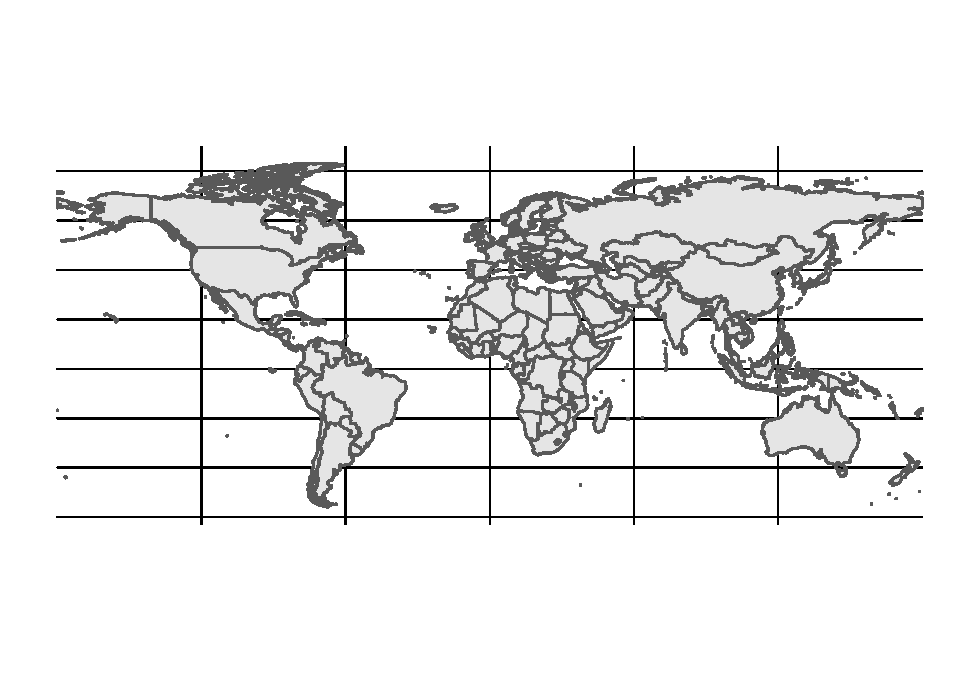
\includegraphics{bachelor-thesis_files/figure-latex/vdem_spatial-1.pdf}
\caption{(\#fig:vdem\_spatial)Country borders in 2017 in the V-Dem
database}
\end{figure}

\begin{itemize}
\tightlist
\item
  \texttt{vdem} which contains the variables from \texttt{df\_vdem}, the
  country shapes from \texttt{vdem\_spatial} and further metainformation
  (see below)
\end{itemize}

Details on these datasets and the reproducible code can be found in the
folder ``data-raw'' in the package.

\section{Package construction}\label{package-construction}

The package has been constructed with the packages \texttt{devtools}
\citep{devtools}, \texttt{roxygen2} \citep{roxygen2} and
\texttt{testthat} \citep{testthat}.

\chapter{Effective explicitness}\label{effective-explicitness}

We describe our methods in this chapter.

\chapter{Applications}\label{applications}

Some \emph{significant} applications are demonstrated in this chapter.

\section{Example one}\label{example-one}

\section{Example two}\label{example-two}

\chapter{Final Words}\label{final-words}

We have finished a nice book.

\bibliography{bachelor-thesis.bib}


\end{document}
